\documentclass{practice}
\usepackage{verbatim}
\usepackage{changepage}

\title{5}
\date{\today}

\begin{document}
\maketitle

\begin{task}{Hlextend}
  Our goal is to very that the MAC construction $t \gets H(k||m)$ for a hash function vulnerable to length-extension attacks is insecure.
  Using SHA256 as the hash function:
  \begin{enumerate}
    \item Create a function \texttt{authenticate(m: bytes) -> bytes} that uses a hardcoded 128-bit random key and returns the authentication tag for the provided message.
    \item Create a function \texttt{verify(m: bytes, t: bytes) -> bool} that uses the same hardcoded 128-bit key to verify the tag on a message.
    \item Choose a message and authenticate it with \texttt{authenticate}.
    Then, using \href{https://github.com/stephenbradshaw/hlextend}{\emph{hlextend}}, forge a tag for a new message.
    Verify your solution using the \texttt{verify} function.
    \item Print the original message and the \enquote{extended} message to the console.
    What do you notice?
  \end{enumerate}

  Which of the following do not hold for this construction: EUF-CMA, EUF-KMA, UUF-CMA, UUF-KMA?
\end{task}

\begin{task}{HMAC}
  Use the python built-in \texttt{hmac} module to generate an authentication tag with HMAC-SHA256.
  Read the module documentation to see how you should verify the MAC.
  What's special about the verification approach?
\end{task}

\begin{task}{Merkle tree}
  For this task, build a binary Merkle tree from the leaf nodes:
  \begin{Verbatim}
["nLkU3/nPBhi/OZRR+b4rknyDWszFvCO1TEkRrbvO6ms=",
 "pP+OvcT4nlZ36CZ9prYB4LIxgFqUHm+x+Lotn78mvOc=",
 "cOdF38vZqJgJINeSnUqz7QAtxlcZOijFGvIqxIXLW1Q=",
 "I6O6kkf6/7jA9P2i6Y0vRKhddV0rEQJunMkOppsmRDA=",
 "GybMHxLyUz16PEXgC0Znr6cCjK9HSJS88S/pqUYhNuc=",
 "V33lVhKtuEAmJGdzoJAa3+hJTentNAnV5F9Prbk5DkA="]
  \end{Verbatim}

  However, notice that the number of leaves is odd, meaning that we cannot build a perfect tree out of these nodes.
  Three different approaches are described at the end of the task.
  Pick one.

  The SHA256 root hash (tree root) should be
  \begin{Verbatim}
J9JWZhuTwTOjS/T+wha5cLd6nyd87/GHv53Ok9Wv94Y= (duplicate last)
zy8NCw9KaWSCWqW6Ulbq76xrB2Jzg7NvhGPCBpiehv8= (promote last)
/o3vEc3FfJD61TqOP0mXzMJnO0lP9N8zvoBjr6K8+nI= (Trillian)
  \end{Verbatim}

  Verify that the string \texttt{A Link to the Past} is included in the tree and provide the proof of inclusion, i.e. the necessary values needed to link the node to the root.

  \textit{Binary Merkle tree construction.}
  Below are three approaches to construct a binary Merkle tree if the number of leaves is not a power of two.
  NB! The first two have subtle issues that are out of our scope.
  Do not blindly use them in production settings.

  \begin{itemize}
    \item Duplicate last leaf -- creates a balanced tree
    
    For every level/row, if the number of nodes is uneven, duplicate the last leaf. E.g.
    \begin{Verbatim}
Level 0:  X1 X2 X3 X4 X5 X5
Level 1:  H1 H2 H3 H3
Level 2:  G1 G2
Level 3:  Root
    \end{Verbatim}
    \item Promote last node -- creates an unbalanced tree
    
    Move the \enquote{extra} node up a level until the level has an even number of nodes. E.g.
    \begin{Verbatim}
Level 0:  X1 X2 X3 X4 X5
Level 1:  H1 H2 X5
Level 2:  G1 X5
Level 3:  Root
    \end{Verbatim}

    \item The Trillian \enquote{tile-based} approach used e.g. by Certificate Transparency (\href{https://datatracker.ietf.org/doc/html/rfc9162#section-2.1.1}{\emph{RFC 6192}}).
    A high level description of the \emph{consistency proofs} this enables can be found \href{https://transparency.dev/verifiable-data-structures/#consistency-proof}{\textit{here}}.
  
    \begin{itemize}
      \item Hash calculations (in RFC 6192) for leaves and nodes differ: they both take a different prefix.
      This is known as domain separation.
      \item The description in the RFC is (in my opinion) quite confusing.
      The tree structure is better illustrated with the following examples:
    \end{itemize}

    \begin{figure}[h!]
    \begin{adjustwidth}{-1.65cm}{-1.65cm}
    \begin{minipage}{0.6\textwidth}
      \centering
      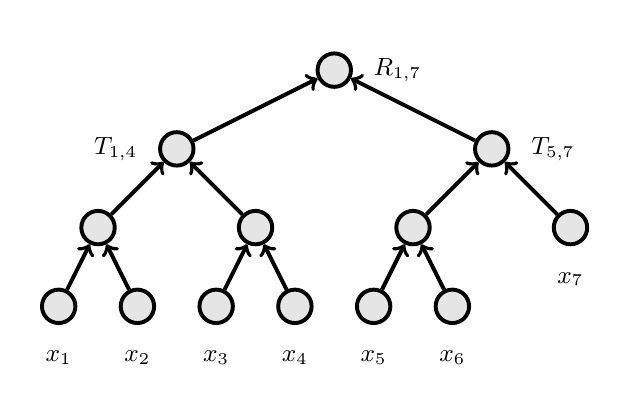
\begin{tikzpicture}
        [level distance=10mm,
        every node/.style={fill=gray!20,draw=black,circle,line width=0.5mm,inner sep=1.5mm},
        edge from parent/.style={<-,draw},
        level 1/.style={sibling distance=40mm,line width=0.5mm,nodes={fill=gray!20}},
        level 2/.style={sibling distance=20mm,nodes={fill=gray!20}},
        level 3/.style={sibling distance=10mm,nodes={fill=gray!20}}]
        \node[label={right:\small $R_{1,7}$}] {}
          child {node[
            label={left:{\small $T_{1,4}$}}] {}
            child {node {}
              child {node[label=south:{\small $x_1$}] {}}
              child {node[label=south:{\small $x_2$}] {}}
            }
            child {node {}
              child {node[label=south:{\small $x_3$}] {}}
              child {node[label=south:{\small $x_4$}] {}}
            }
          }
          child {node[label={right:\small $T_{5,7}$}] {}
            child {node {}
              child {node[label=south:{\small $x_5$}] {}}
              child {node[label=south:{\small $x_6$}] {}}
            }
            child {node[label={south:\small $x_7$}] {}}
          };
      \end{tikzpicture}
    \caption{Trillian Merkle tree with 7 leaves, resulting in an unbalanced tree.
    The tiles are split at $k=4$ since it is the largest power of two $< 7$.}
    \end{minipage}
    \hfill
    \begin{minipage}{0.6\textwidth}
      \centering
      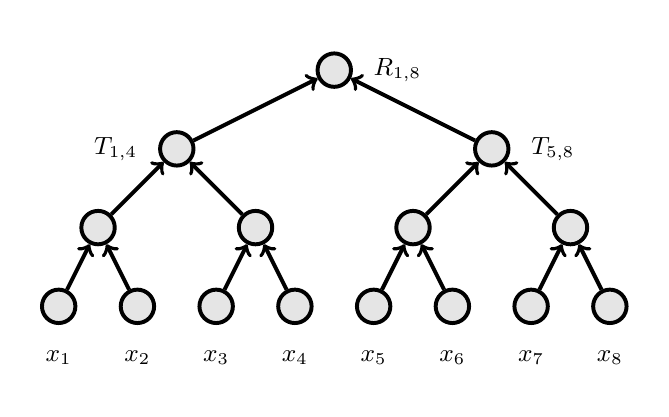
\begin{tikzpicture}
        [level distance=10mm,
        every node/.style={fill=gray!20,draw=black,circle,line width=0.5mm,inner sep=1.5mm},
        edge from parent/.style={<-,draw},
        level 1/.style={sibling distance=40mm,line width=0.5mm,nodes={fill=gray!20}},
        level 2/.style={sibling distance=20mm,nodes={fill=gray!20}},
        level 3/.style={sibling distance=10mm,nodes={fill=gray!20}}]
        \node[label={right:\small $R_{1,8}$}] {}
          child {node[
            label={left:{\small $T_{1,4}$}}] {}
            child {node {}
              child {node[label=south:{\small $x_1$}] {}}
              child {node[label=south:{\small $x_2$}] {}}
            }
            child {node {}
              child {node[label=south:{\small $x_3$}] {}}
              child {node[label=south:{\small $x_4$}] {}}
            }
          }
          child {node[label={right:\small $T_{5,8}$}] {}
            child {node {}
              child {node[label=south:{\small $x_5$}] {}}
              child {node[label=south:{\small $x_6$}] {}}
            }
            child {node {}
              child {node[label=south:{\small $x_7$}] {}}
              child {node[label=south:{\small $x_8$}] {}}
            }
          };
        \end{tikzpicture}
    \caption{After appending the 8th node to the Trillian tree, the tree is now balanced.
    The left subtree remains unchanged.}
    \end{minipage}
    \end{adjustwidth}
    \end{figure}
  \end{itemize}
\end{task}

\end{document}
